%%%%%%%%%%%%%%%%%%%%%%%%%%%%%%%%%%%%%%%%%
% Thin Sectioned Essay
% LaTeX Template
% Version 1.0 (3/8/13)
%
% This template has been downloaded from:
% http://www.LaTeXTemplates.com
%
% Original Author:
% Nicolas Diaz (nsdiaz@uc.cl) with extensive modifications by:
% Vel (vel@latextemplates.com)
%
% License:
% CC BY-NC-SA 3.0 (http://creativecommons.org/licenses/by-nc-sa/3.0/)
%
%%%%%%%%%%%%%%%%%%%%%%%%%%%%%%%%%%%%%%%%%

%----------------------------------------------------------------------------------------
%	PACKAGES AND OTHER DOCUMENT CONFIGURATIONS
%----------------------------------------------------------------------------------------

\documentclass[a4paper, 11pt]{article} % Font size (can be 10pt, 11pt or 12pt) and paper size (remove a4paper for US letter paper)

\usepackage[protrusion=true,expansion=true]{microtype} % Better typography
\usepackage{graphicx} % Required for including pictures
\usepackage{wrapfig} % Allows in-line images
\usepackage{amsmath} % Import math module
\usepackage{float} % For positioning the figures

\usepackage[labelfont=bf,font=small,font=it]{caption} % Bold the figure label and make it smaller
\usepackage[none]{hyphenat} % Prevent hyphenation 

\usepackage{mathpazo} % Use the Palatino font
\usepackage[T1]{fontenc} % Required for accented characters
\usepackage[utf8]{inputenc} % for the bibliography
\linespread{1.50} % Change line spacing here, Palatino benefits from a slight increase by default

\makeatletter
\renewcommand{\@listI}{\itemsep=0pt} % Reduce the space between items in the itemize and enumerate environments and the bibliography

\renewcommand{\maketitle}{ % Customize the title - do not edit title and author name here, see the TITLE block below
\begin{flushright} % Right align
{\LARGE\@title} % Increase the font size of the title

\vspace{20pt} % Some vertical space between the title and author name

{\large\@author} % Author name
\\\@date % Date

%\vspace{40pt} % Some vertical space between the author block and abstract
\end{flushright}
}

% setting up the various tittle formats % 
\usepackage{titlesec}
\titleformat*{\section}{\fontsize{16}{19}\bfseries}
\titleformat*{\subsection}{\fontsize{14}{17}\bfseries}
\titleformat*{\subsubsection}{\fontsize{12}{17}\itshape}

%----------------------------------------------------------------------------------------
%	TITLE
%----------------------------------------------------------------------------------------

\title{\textbf{Where's Waldo?}\\ % Title
 Modeling Autonomous Search} % Subtitle

\author{\textsc{Claudine LeBosquain} % Author
\\{260449697}%
\\{\textit{COMP 417 Term Paper}}} % Institution

\date{December 14, 2014} % Date

%----------------------------------------------------------------------------------------

\begin{document}

\maketitle % Print the title section

%----------------------------------------------------------------------------------------
%	ESSAY BODY
%----------------------------------------------------------------------------------------

\section*{Introduction}

The popular children's book series "Where's Waldo?" involves searching for a character named Waldo, who is hidden among many other people, a few of whom possess some of Waldo's characteristic features. This "search for a target" theme is shared with the burgeoning field of autonomous robot rendezvous in which only one of the robots has control over its speed and velocity. The present work aims to investigate the time taken for an autonomous aquatic robot to locate an object adrift at sea (thought the methods employed should theoretically be applicable to similar situations at any scale). This task shares many problems which are also apparent in the remarkably frustrating process of trying to find Waldo, including a noisy environment, and characteristic features of the target, and a limited (though variable) world size. Despite these similarities, there are also some notable differences. The two most important of these differences are: 
\begin{enumerate}
\item \textbf{We know where the target begins and have an idea where it goes.} In "Where's Waldo?" the children are not given a start point. Waldo could be anywhere on the page. In the problem that I will be considering in this paper, the robot begins knowing where the target was released, so it has a general idea about where to begin looking. Additionally, have a general idea of where the target might be in the future (in the form of a probability distribution). This makes our problem slightly easier. 
\item \textbf{The target moves.} "Where's Waldo?" is a book, and unfortunately, in our mundane, magic-free world, the pictures do not move. In real life, however, and especially in an ocean, the target does not remain stationary with the passage of time - the analogy equivalent of a "wandering Waldo". We must take this into account when searching for the object, which presents a slight complication.
\end{enumerate} 

%------------------------------------------------

\section*{Background and Related Work}

Robot rendezvous is an up-and-coming field of research in the robotics community. Publications regarding robot rendezvous have covered a wide range of possible scenarios. The majority of the research seems to be centred around robots who are in constant communication via sight~\cite{Rekleitis2001c}, a network of radio beacons~\cite{batalin2004}, or other unspecified means~\cite{burgard2000}\cite{rekleitis20082}. Work has even been done to compare different methods of communication~\cite{rekleitis20081}. However, a portion of this field remains dedicated to investigating independently exploring robots which cannot remain in constant communication due to a limited communication radius. Basic concepts introduced by various authors~\cite{Dudek97AAAIw}\cite{Roy2000}, have recently been extended to a real-world challenge involving an autonomous underwater vehicle (AUV) which is attempting to locate and exchange information with a free-floating drifter with a limited communication radius due to radio signal attenuation under water~\cite{meghjani14}. \\

\noindent Currently, no work has been done regarding the total time taken for a robot to locate a drifter. This is what I aim to explore in this paper. I begin with a basic model in which the robot heads directly to the most likely location of the drifter. The most likely location is determined by the AUV's probabilistic model of the drifter's movement. Meghjani et al. ~\cite{meghjani14} discuss using spiral search patterns to locate the drifter, which have proven to be the optimal search strategy with no information ~\cite{alpern2003}. I attempt to incorporate this into my model using a square spiral search pattern. Furthermore, the basic model is competent framework which is well suited to future additions and improvements to the model. 

%------------------------------------------------

\section*{Method Used}

The problem presented in this paper regarding robot rendezvous at sea has three main components - the body of water (the ocean), the robot (AUV), and the sensor or beacon (drifter). The ocean, or search space, is represented as a square 2D array of floating point numbers. These correspond to probabilities which reflect the robot's belief regarding the sensor's location. Each unit represents 1 $m$. Throughout the paper, the size of the search space will refer to the length of the array. For example, a search space of size 100 $m$ will be represented by a 100 $m$ by 100 $m$ array of floats. The robot can detect the beacon if it is within a 5 unit radius (in other words, the communication radius, $R_{comm}$ is 5 $m$ as suggested in ~\cite{meghjani14}). The drift probability of the sensor is modelled by a kernel which undergoes convolution with the ocean at each time step. 
\\

\noindent At $t=0$ the drifter is placed in a location in the ocean, and this location in the array is set to $1.0$ seeing as the probability of the robot being in this location at $t=0$ is $1.0$. At each subsequent time step $t=n$, we convolve the ocean and the kernel to produce a new belief state for the robot. Then, we plan the action the robot should take, execute this action, check for the drifter, update the belief state and then begin the whole process over again at $t=n+1$. These sections will be discussed in greater detail below. \\

\noindent The current work considers 3 models: 
\begin{enumerate}
\item \textbf{The Basic Model} in which the drifter moves randomly according to a uniform distribution. The drifter begins in the middle of the world and the AUV starts at position (0,0). 
\item \textbf{The Randomized-Basic Model} which extends the Basic Model by simply randomizing the starting locations of both the AUV and the drifter, resulting in variable initial distances between the AUV and drifter.
\item \textbf{The Square Spiral Model:} which extends the Randomized-Basic model by implementing a square spiral upon reaching the highest probability location and failing to find the drifter.
\end{enumerate}

\subsection*{Convolution}

\begin{wrapfigure}{rh}{0.5\textwidth}
	\vspace{-40pt}
	\begin{center}
		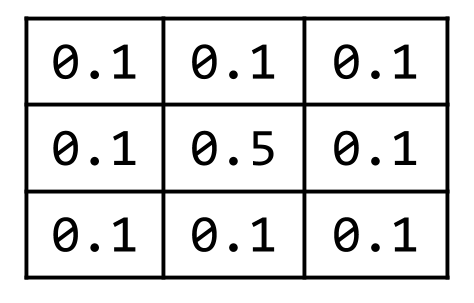
\includegraphics[scale=0.30]{Basic_Kernel.png}
		\vspace{-20pt}
	\end{center}
\caption{Kernel used in the all models \label{basicKernel}}
\vspace{-10pt}
\end{wrapfigure}

In all models considered in this paper, the AUV's estimation of the drifter's movement is defined by a 3x3 kernel, which can be seen in Figure~\ref{basicKernel}. At each time step, this kernel undergoes convolution with the 2D array of floats representing the current belief AUV has about the drifter's location.

\subsection*{Planning the Action}

The action phase depends largely on the speed of the AUV. In previous work by Meghjani et al.~\cite{meghjani14}, it is mentioned that the AUV has a speed of approximately 1 $m/s$, so we allow the AUV to move 1 $m$ per time increment and thus all times are measured in seconds. 

\subsubsection*{Basic and Randomized-Basic Models}

In the Basic and Randomized Basic models, we calculate the difference between the $x$ and $y$ coordinates of the most likely location of the drifter and the current location of the AUV. Using the basic geometry rules presented in Figure~\ref{basicGeo2} and Figure~\ref{basicGeo1}, we are able to compute how far the AUV should move along the $x$ and $y$ axes to ensure that the magnitude of the hypotenuse remains at 1 (the maximum speed of the AUV). We do this by first calculating the magnitude of $x_{distance}$ and $y_{distance}$, and then calculating $\theta$ by recalling that $\theta = \arctan{\frac{x_{distance}}{y_{distance}}}$. Once we have calculated $\theta$ and modified it to reflect the correct angle (Figure~\ref{basicGeo2}) , we can calculate the $x$ and $y$ values of the similar triangle with hypotenuse of length 1, which are the values we need to add to our current $x$ and $y$ position (Figure~\ref{basicGeo1}).

\begin{figure}[H]
	\begin{center}
		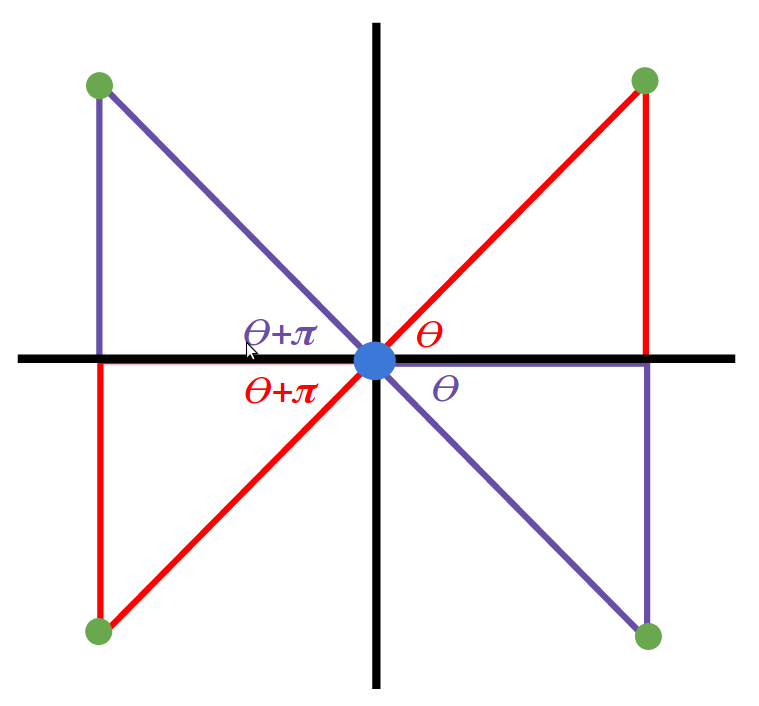
\includegraphics[scale=0.20]{angles.png}
	\end{center}
\caption{Addition of pi to obtain the correct angle \label{basicGeo2}}
\end{figure}

\begin{figure}[H]
	\begin{center}
		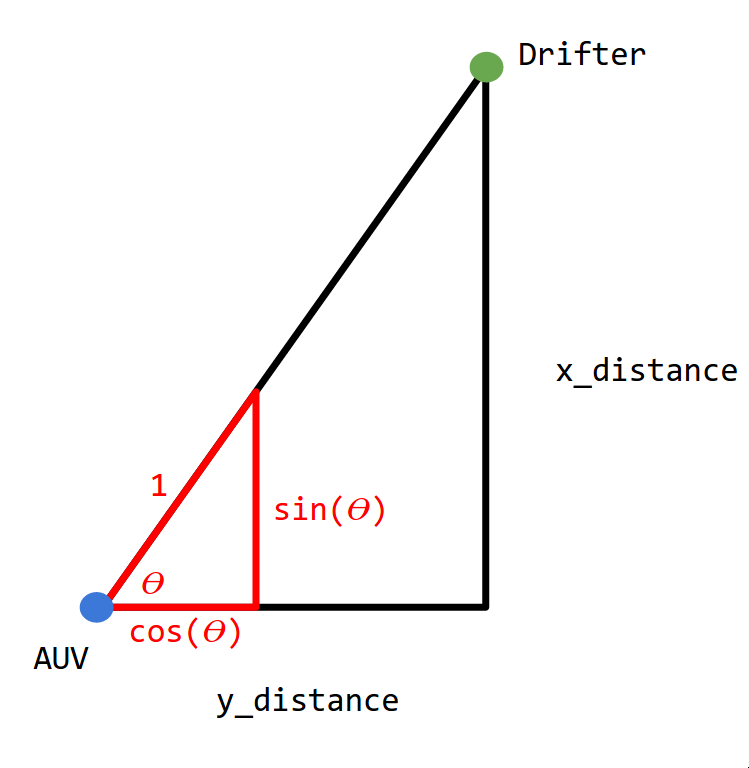
\includegraphics[scale=0.20]{distance_calculation.png}
	\end{center}
\caption{Calculating change in $x$ and $y$ for the AUV \label{basicGeo1}}
\end{figure}

\subsubsection*{Square Spiral Model}

The Square Spiral Model differs from the Basic and Randomized Basic Models when the coordinates of the highest probability location changes. The only reason that these coordinates would change is that the AUV has passed near by, checked this location, failed to find the drifter and set the probability to 0 (see the Observation and Update section for further detail). 

\begin{wrapfigure}{rh}{0.5\textwidth}
	\vspace{-20pt}
	\begin{center}
		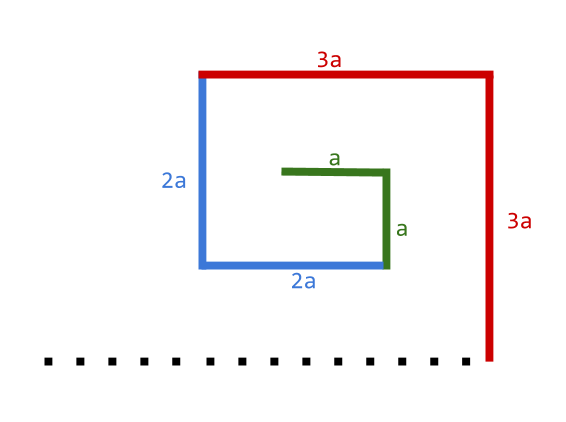
\includegraphics[scale=0.30]{spiral.png}
		\vspace{-20pt}
	\end{center}
\caption{Spiral, $R_{comm} = a$ \label{spiral}}

\end{wrapfigure}

\noindent In the Square Spiral, the AUV realizes that it is close to where the drifter should be, but that it has not yet found the drifter and decides to initiate a square spiral search pattern to search the area more thoroughly. This is in direct contrast to the Basic and Randomized Basic models which, in the same scenario, would simply have the AUV blindly begin moving toward the new highest probability location.\\

\noindent The specifications of the spiral can be seen in Figure ~\ref{spiral}. This spiral is defined by first heading right, then down, then left, and finally up. This order is pre-specified, as is the amount we increase the side lengths by. The variable "a" in the spiral pictured in Figure ~\ref{spiral} refers to the size of the communication range in which the robot can safely detect presence of the drifting beacon. This ensures that the spiral search covers all the area and does not leave any gaps. Once a spiral has been initiated, the spiral pattern persists until the drifter is found. 

\subsection*{Observation and Update}

In all models, when looking for the drifter, the model will calculate the Euclidean distance between the AUV and the drifter:

\begin{equation*}
d(beacon,AUV) = \sqrt{(beacon_{x} - AUV_{x})^{2} - (beacon_{y} - AUV_{y})^{2})}
\end{equation*} 

\noindent If the distance between the drifter and the AUV is less than 5 $m$, the simulation ends and returns the time to find the drifter. 

\noindent However, if the drifter does not fall within the communication radius, the probabilities of the array cells surrounding the AUV in a radius of 4 are set to zero. \\

\noindent We cannot set the all cells in radius 5 around the AUV to 0 because if the distance is just a little bit more of the 5 $m$ radius but is on an angle so that it is still located within that 5th cell, we don't want it to be set to zero. This can be seen in Figure~\ref{wrongToZero}. Once this probability resetting is complete, the process will repeat again with the convolution step, and the timer counter will be incremented by one.

\begin{figure}[H]
	\vspace{-20pt}
	\begin{center}
		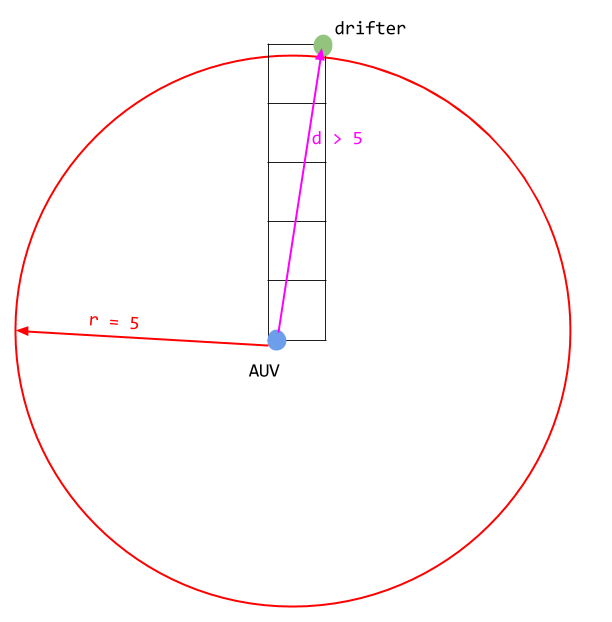
\includegraphics[scale=0.30]{wrongToZero.png}
		\vspace{-20pt}
	\end{center}
\caption{$R_{comm} = 5$, but the distance from the AUV to the drifter, $d$, is greater than 5. All 5 of the grid squares would be (incorrectly) labelled with probability 0 and the robot would move away from this area. \label{wrongToZero}}
\vspace{10pt}
\end{figure}

%------------------------------------------------

\section*{Experimental Results}


\subsection*{Basic Model} 

In the basic model as described above, with a world size of 100 $m$ by 100 $m$, after 1000 trials, the average time it takes for the AUV to find the drifter is 64.904 seconds. In other words, a drifter located approximately 70.0 $m$ away (which can easily be found using the Pythagorean theorem and the knowledge that the drifter begins at the center of a 100 $m$ by 100 $m$ grid, and the AUV begins at location (0,0)) the drifter is located after just over a minute of search. A trial is shown in Figure ~\ref{basicAUVDrifer} and  closer look at the motion of the drifter is presented in Figure ~\ref{basicDriferCloseup}.   

\begin{figure}[H]
	\begin{center}
		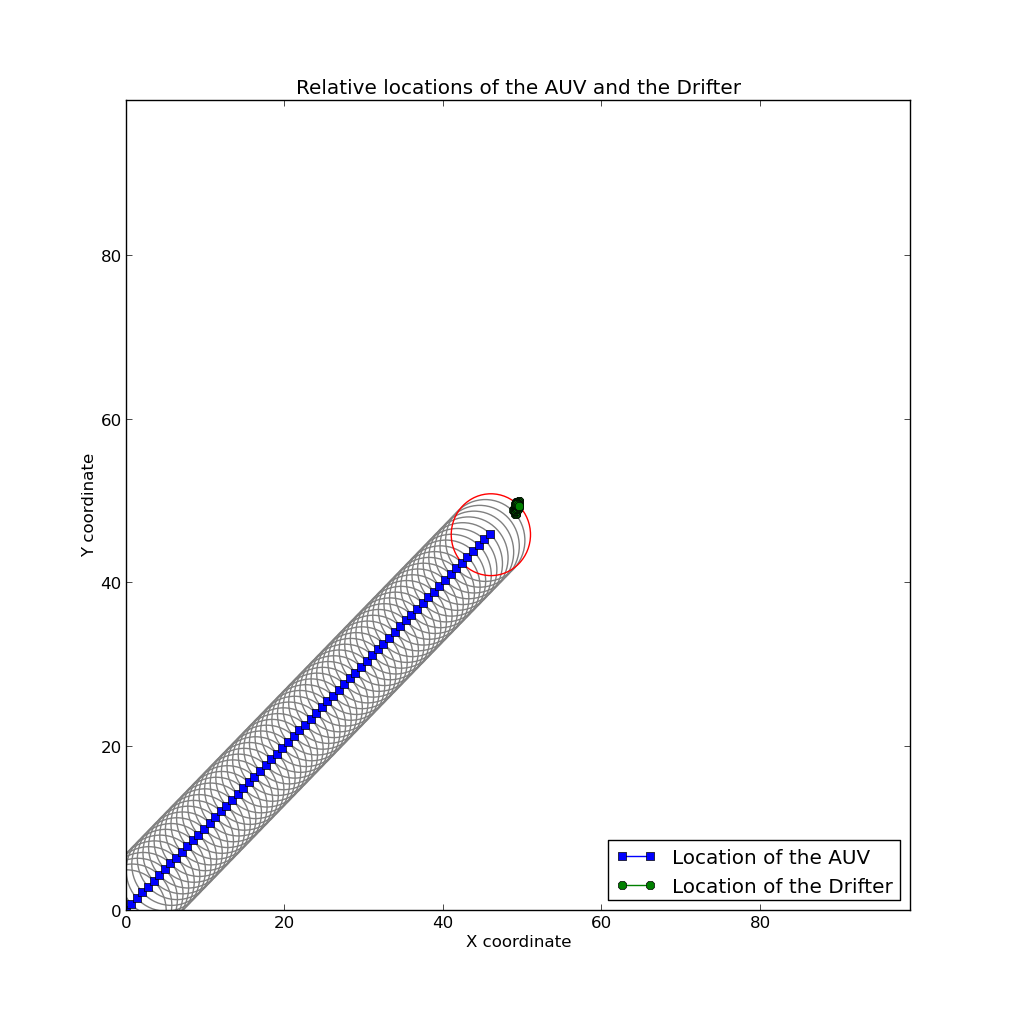
\includegraphics[scale=0.30]{basic_1.png}
	\end{center}
\caption{Motion of AUV and drifter. Grey circles represent the $R_{comm}$ of the AUV and the red circle is the final $R_{comm}$ in which drifter was found. \label{basicAUVDrifer}}
\end{figure}

\begin{figure}[H]
	\begin{center}
		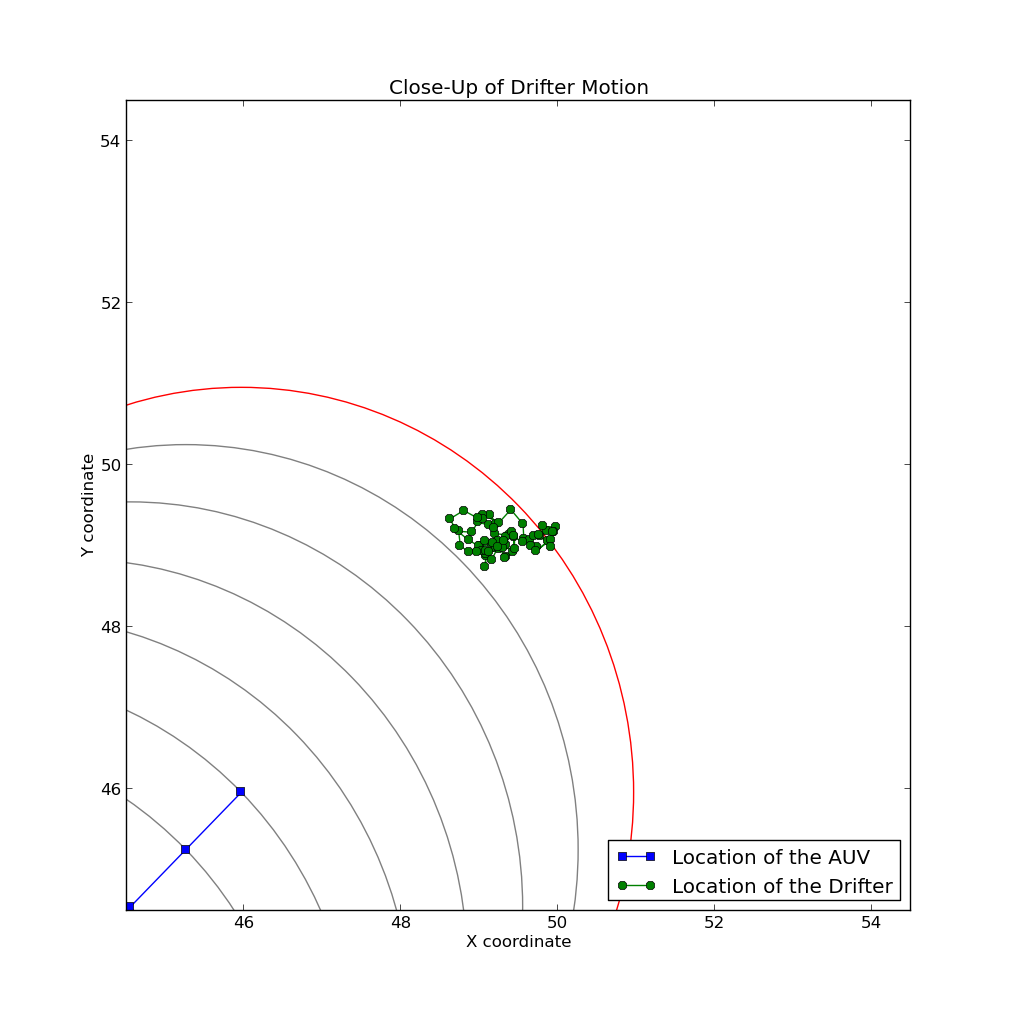
\includegraphics[scale=0.30]{basic_2.png}
	\end{center}
\caption{Close-Up of drifter motion. As before, grey circles represent the $R_{comm}$ of the AUV and the red circle is the final $R_{comm}$ in which drifter was found. \label{basicDriferCloseup}}
\end{figure}

\noindent We can expand this model slightly by playing with the parameters. What happens to the search time as we increase the size of the world? Figure ~\ref{timeIncrease} shows the plot of search time as the size of the search space increases from 50 $m$ to 500 $m$ (ie. 2500 $m^2$ to 250000 $m^2$). We can see that the search time increase appears to be linear. 

\begin{figure}[H]
	\begin{center}
		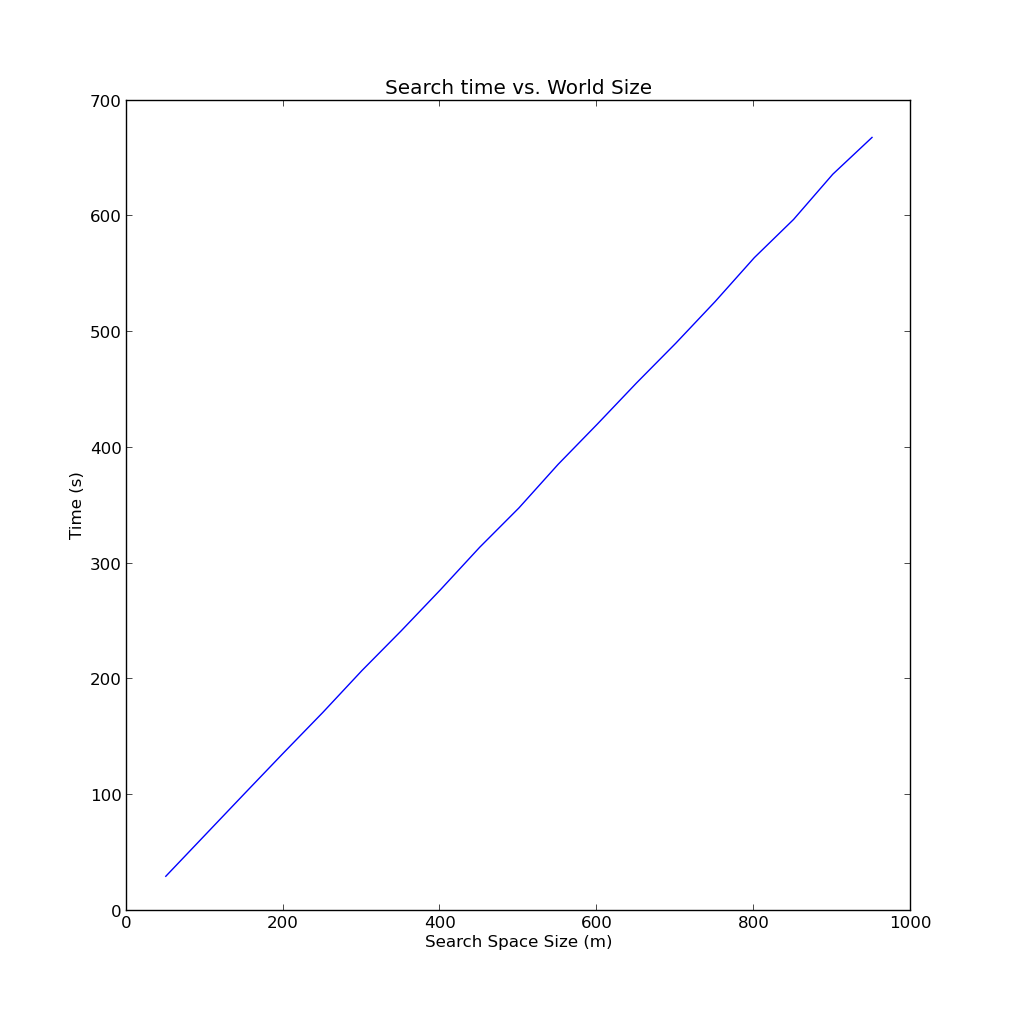
\includegraphics[scale=0.30]{basic_3.png}
	\end{center}
\caption{Search Time as World Size Increases \label{timeIncrease}}
\end{figure}

\noindent However, upon testing the Randomized-Basic model, it becomes very clear that there is a problem with the method. Frequently the AUV comes close to the drifter but fails to find it, moves away, and never comes back to the area. This problem is exemplified in Figure ~\ref{failureToLocate}. Clearly, the robot approaches the drifter and in fact gets very close. However, upon getting close to the maximum probability location it sets the probabilities in the communication radius to 0. This often results in setting the probability of the most likely location to 0. The AUV then moves off in the wrong direction and never manages to locate the drifter. This makes clear the need for a spiral-out search method - when the AUV approaches the location where the drifter is most likely to be but fails to find the drifter, instead of blindly moving to the next most probable area (which might very well mean moving away from the drifter), it makes more sense to spiral outward from the current location, searching in the area until it locates the drifter.

\begin{figure}[H]
	\begin{center}
		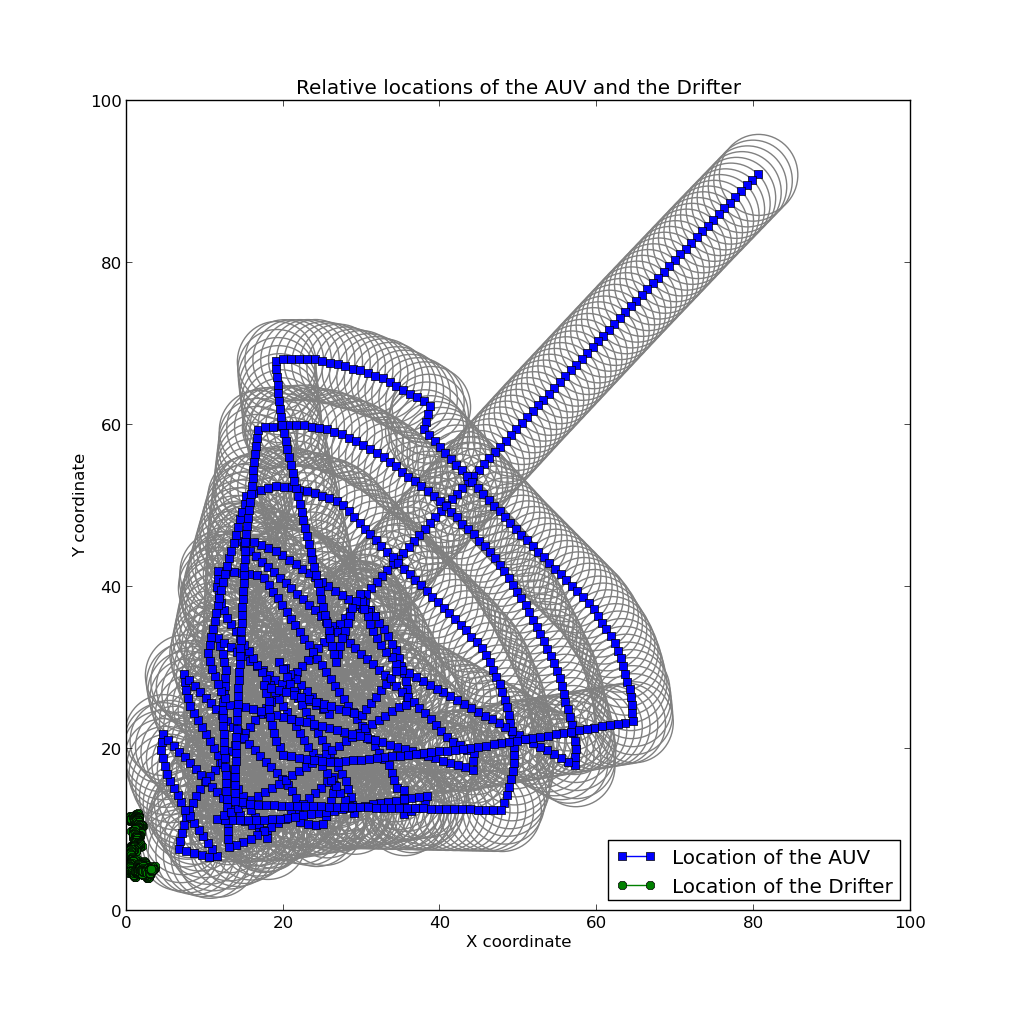
\includegraphics[scale=0.30]{basic_4.png}
	\end{center}
\caption{AUV Fails to Find the Drifter \label{failureToLocate}}
\end{figure}

\noindent Unfortunately because of these failure cases, which occurred quite often, we were unable to obtain a graph of the time it took to find the drifter as a function of the random initial distances.

\subsection*{Square Spiral Outward}

The Square Spiral Outward shows much better results than the Randomized-Basic model. It is more succesful in finding the drifter (though it does fail occasionally, see the Critique for more information). We can see examples of the formation of a spiral in Figure~\ref{exampleSpiral100} for a search space of 100 $m$, and Figure~\ref{exampleSpiral200} for a search space of 200 $m$.  

\begin{figure}[H]
	\begin{center}
		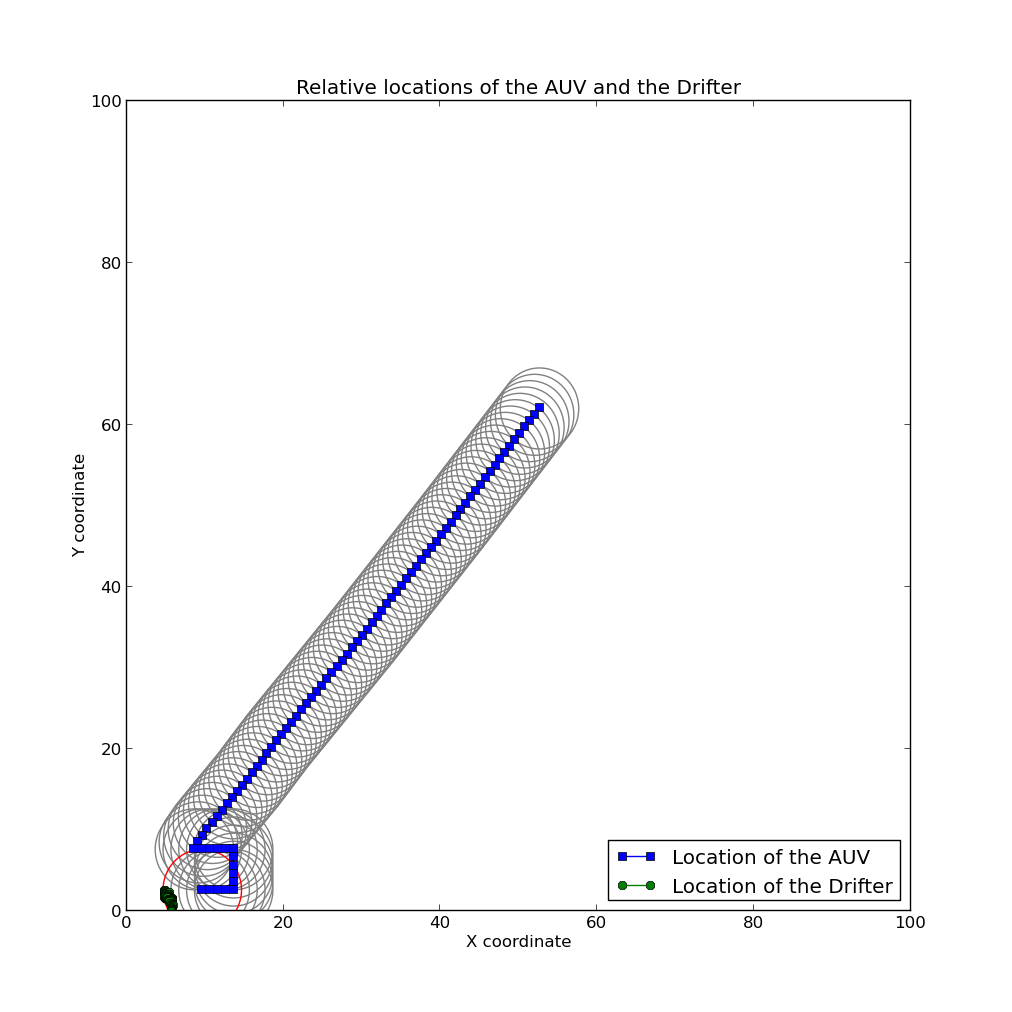
\includegraphics[scale=0.30]{example_spiral_1.png}
	\end{center}
\caption{Example of a Spiral Formation\\ ($R_{comm}$= 5$m$, World Size = 100 $m$) \label{exampleSpiral100}}
\end{figure}

\begin{figure}[H]
	\begin{center}
		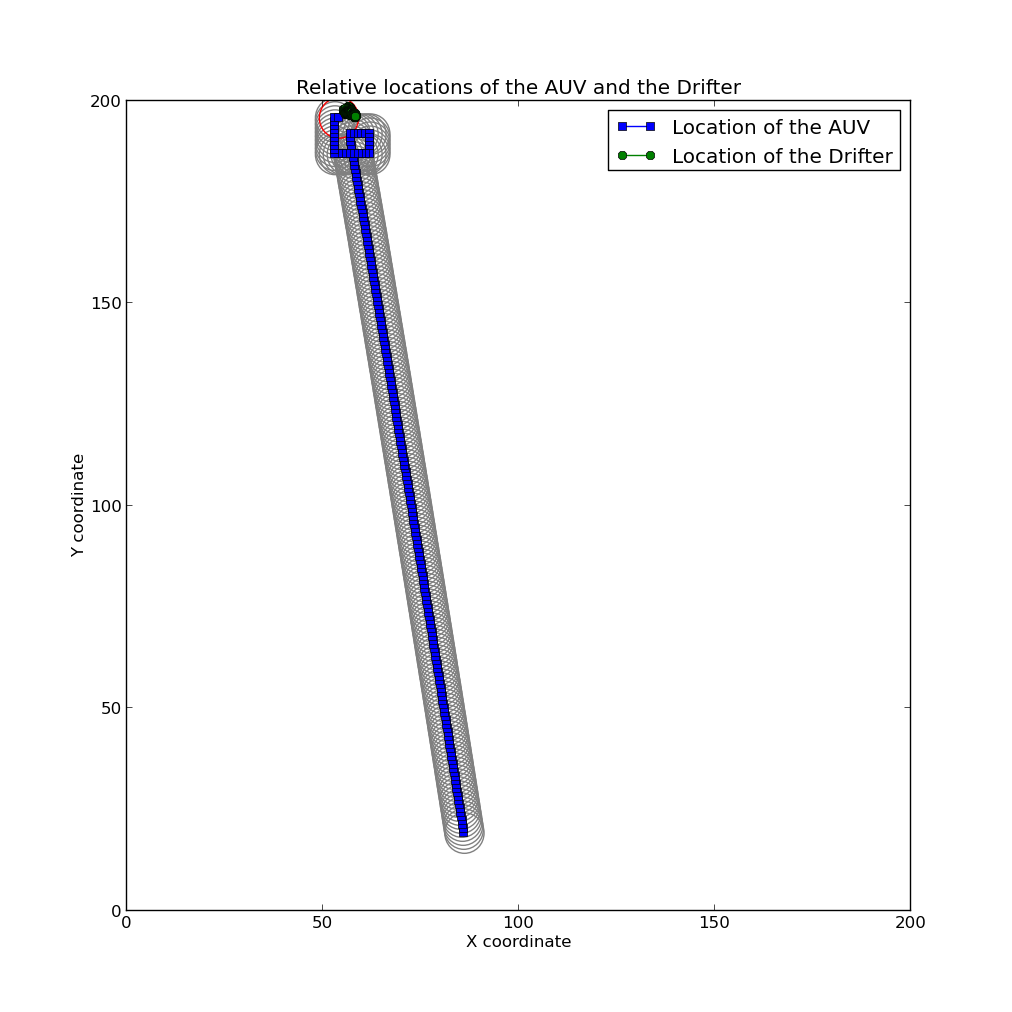
\includegraphics[scale=0.30]{example_spiral_2.png}
	\end{center}
\caption{Example of a Spiral Formation\\ ($R_{comm}$= 5$m$, World Size = 200 $m$) \label{exampleSpiral200}}
\end{figure}

\noindent After running 100 trials of the Square Spiral Outward, we can make a plot of the initial distance with respect to the time it took to find the drifter, as seen in Figure ~\ref{distanceVTime5}. The points that lie mostly along the line represent the cases which were found simply by approaching the highest probability location, and which did not need to spiral. The points that exhibit high values for the time taken are those that had to undergo spiralling to find the drifter. The longer the spiral persisted, the longer it took to find the drifter. After computing 100 plots, we compute the the average slope is 1.06 and the average intercept is -6.33 leading to a line of best fit represented by $y= 1.06x - 6.33$. The average miss rate is 0.12\%.\\

\begin{figure}[H]

	\begin{center}
		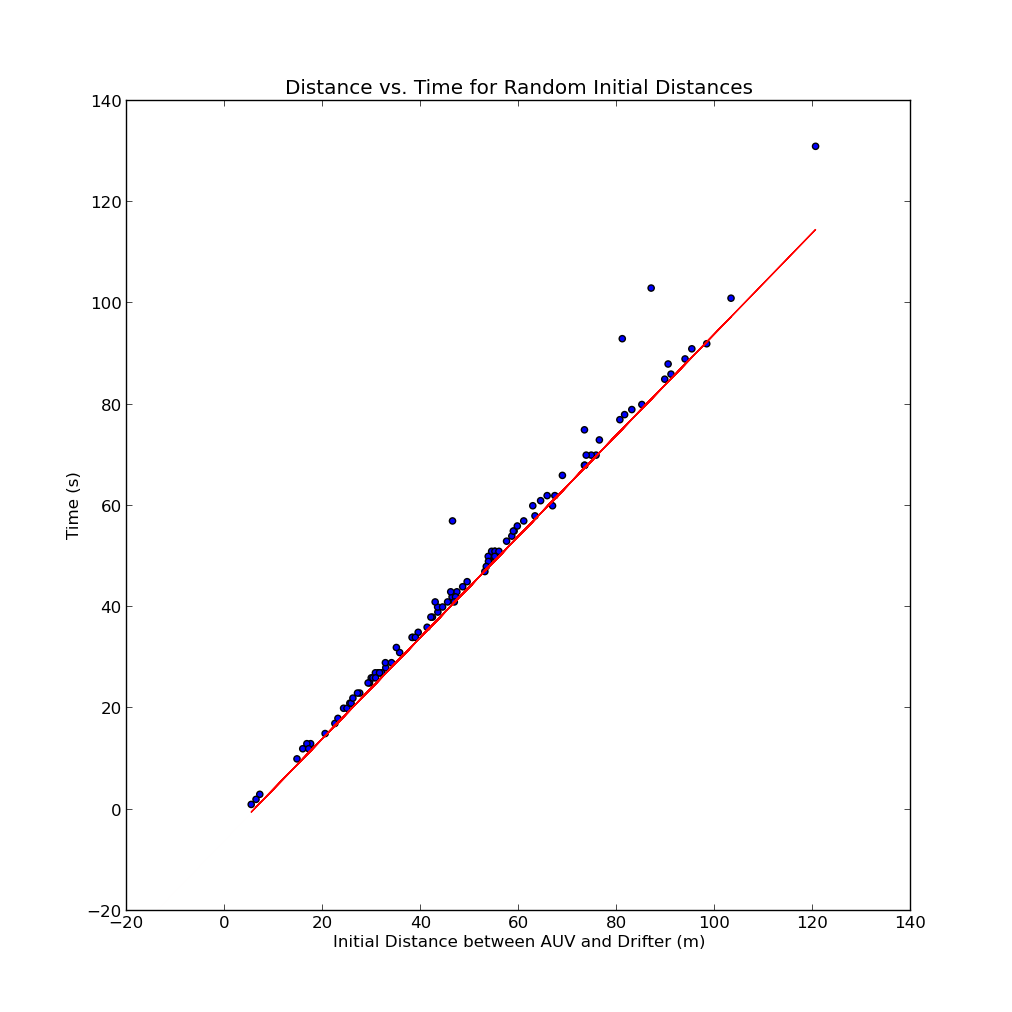
\includegraphics[scale=0.30]{distance_calculation_rcomm5.png}
	\end{center}
\caption{Initial Distance vs. Time Taken to Find the Drifter\\ ($R_{comm}$= 5$m$, World Size = 100 $m$) \label{distanceVTime5}}
\end{figure}

\noindent We can also reduce the communication radius to demonstrate more fully developed spirals, and simulate search in a larger world. This is accomplished by making the communication radius relatively smaller as opposed to making the world size relatively larger. \\

\noindent With a communication radius of 2.5 $m$ (while setting probabilities of squares in a radius of 2 around the robot to 0), and a world size of 200 $m$, we we managed to achieve the spiral seen in Figure ~\ref{complexSpiral2.5}. Setting the world size to 100 $m$ and plotting the initial distance vs. time taken, we obtain the plot seen in ~\ref{distanceVTime2.5}. The interpretation of this graph is the same as the interpretation of the Figure ~\ref{distanceVTime5}. After computing 100 plots, we find the average slope is 1.10 and the average intercept is -4.76 leading to a line of best fit represented by $y = 1.10x - 4.76$. Trials in which the AUV fails to find the drifter were excluded from the calculation. The average miss rate is 0.19\%. \\

\noindent When comparing the distance vs. time graphs for both $R_{comm} = 5$ and $R_{comm} =2.5$, we can see that both show more deviation from the line of best fit as the initial distance grows. This is expected, because if there is a larger initial distance, it takes longer for the AUV to reach the point of highest probibility, and thus the drifter has had more time to move away from this location. The graphs have nearly the same slope, which is consistent with the idea that these are the trials in which the drifter can be found simply by going to the highest-probability location. The fact that the slope is steeper for the smaller communication radius indicates that it takes longer to find the drifter with a smaller communication radius. This explains the higher miss rate when using a smaller communication radius - when the communication radius is smaller it takes longer to find the drifter and gives the drifter more time to move back into space that has already been covered by the spiral. It is important to remember that each of these graphs are built upon a set of 100 trials, but since each trial is random, the graphs are different every time. 

\begin{figure}[H]
	\begin{center}
		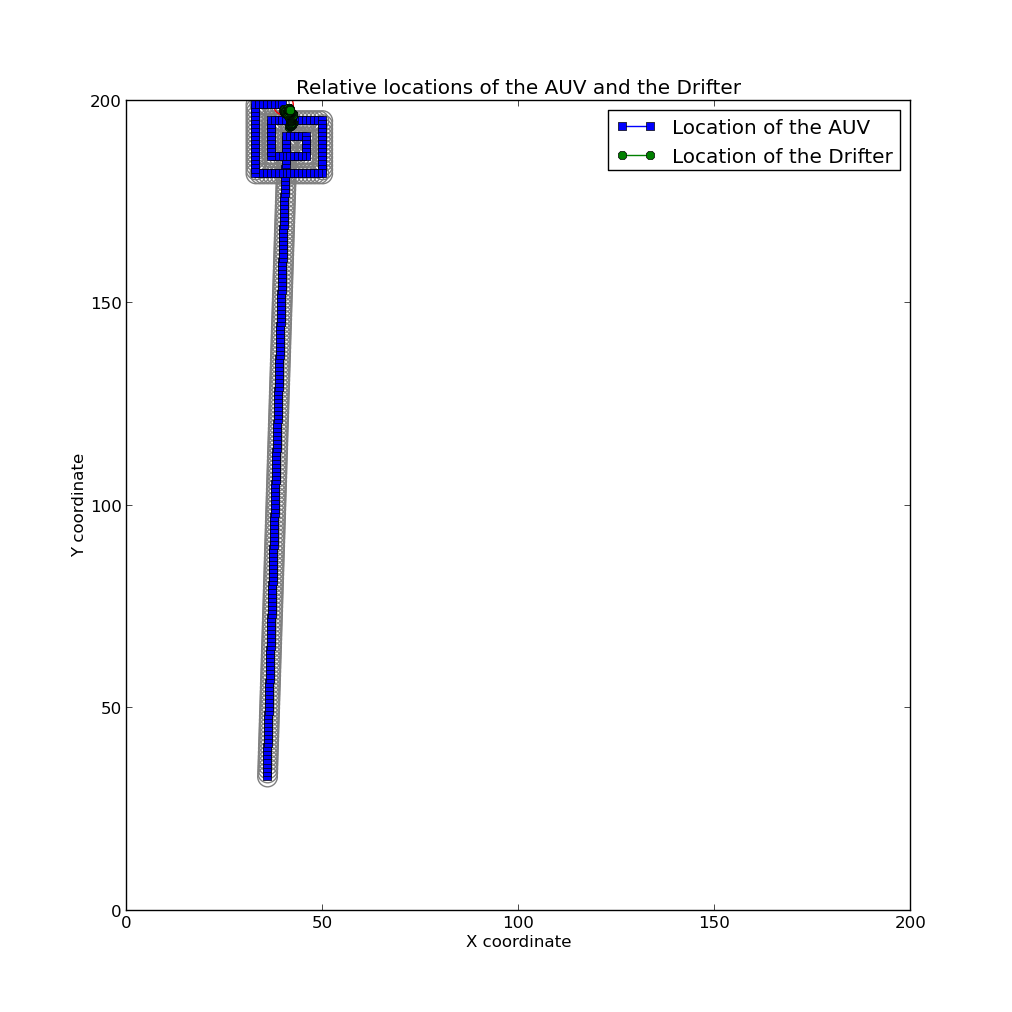
\includegraphics[scale=0.30]{rcomm25_1.png}
	\end{center}
\caption{Example of a more complex spiral formation\\ ($R_{comm}$= 2.5$m$, World Size = 200 $m$) \label{complexSpiral2.5}}
\end{figure}

\begin{figure}[H]
	\begin{center}
		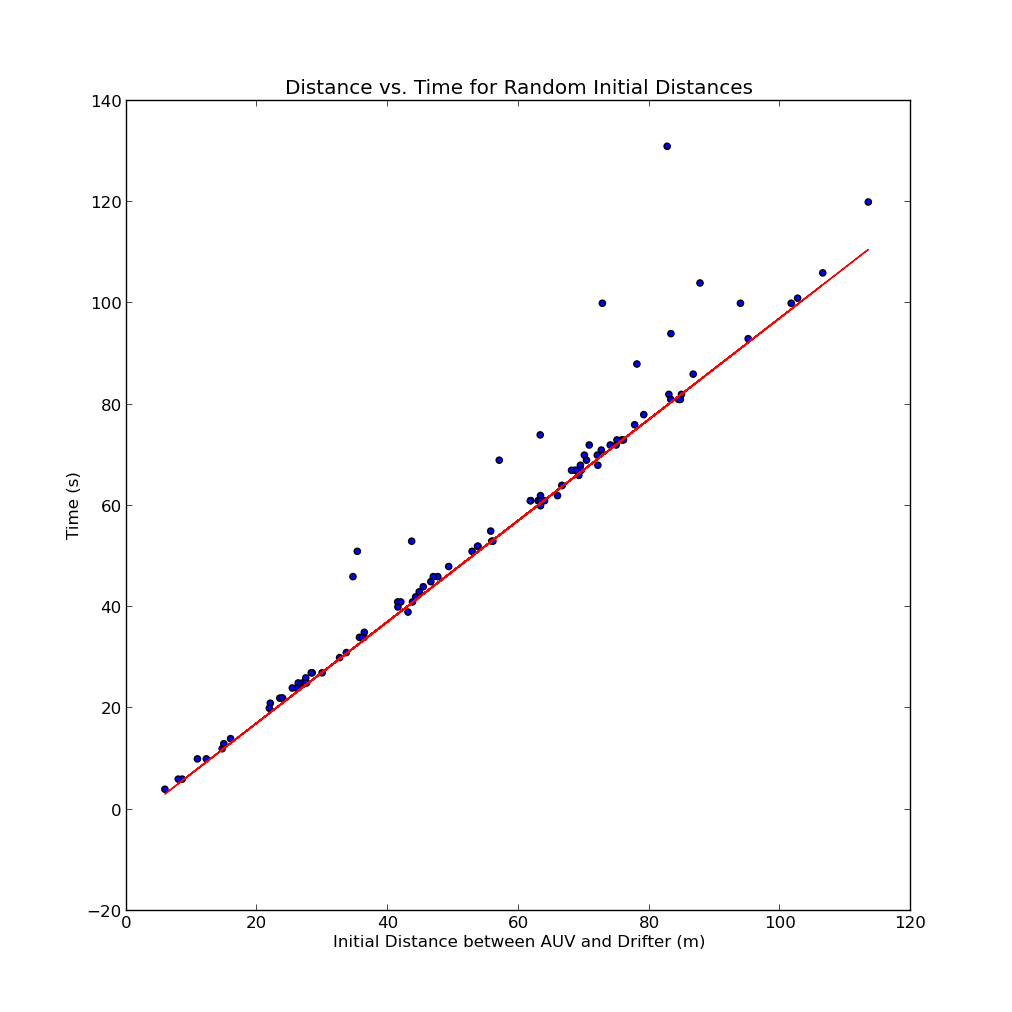
\includegraphics[scale=0.30]{distance_calculation_rcomm25.png}
	\end{center}
\caption{Initial Distance vs. Time Taken to Find the Drifter\\ ($R_{comm}$=2.5$m$, World Size = 100 $m$) \label{distanceVTime2.5}}
\end{figure}
%------------------------------------------------

\section*{Critique of Method}

It is worth noting that the spiral that we are using is not always the most efficient. In many cases, it doubles back on territory previously covered in the AUV's movement toward the most likely location (see Figure ~\ref{badSpiral}). Because of the way we have coded the spiral to always begin by going to the right, then down, then left, and finally up and then repeating the cycle, it is not able to adapt to its circumstances. A prudent, effiencency-improving modification would be to have the first spiral step head in the direction of the current most probable location, and then spiral out from there. \\

\begin{figure}[H]
	\begin{center}
		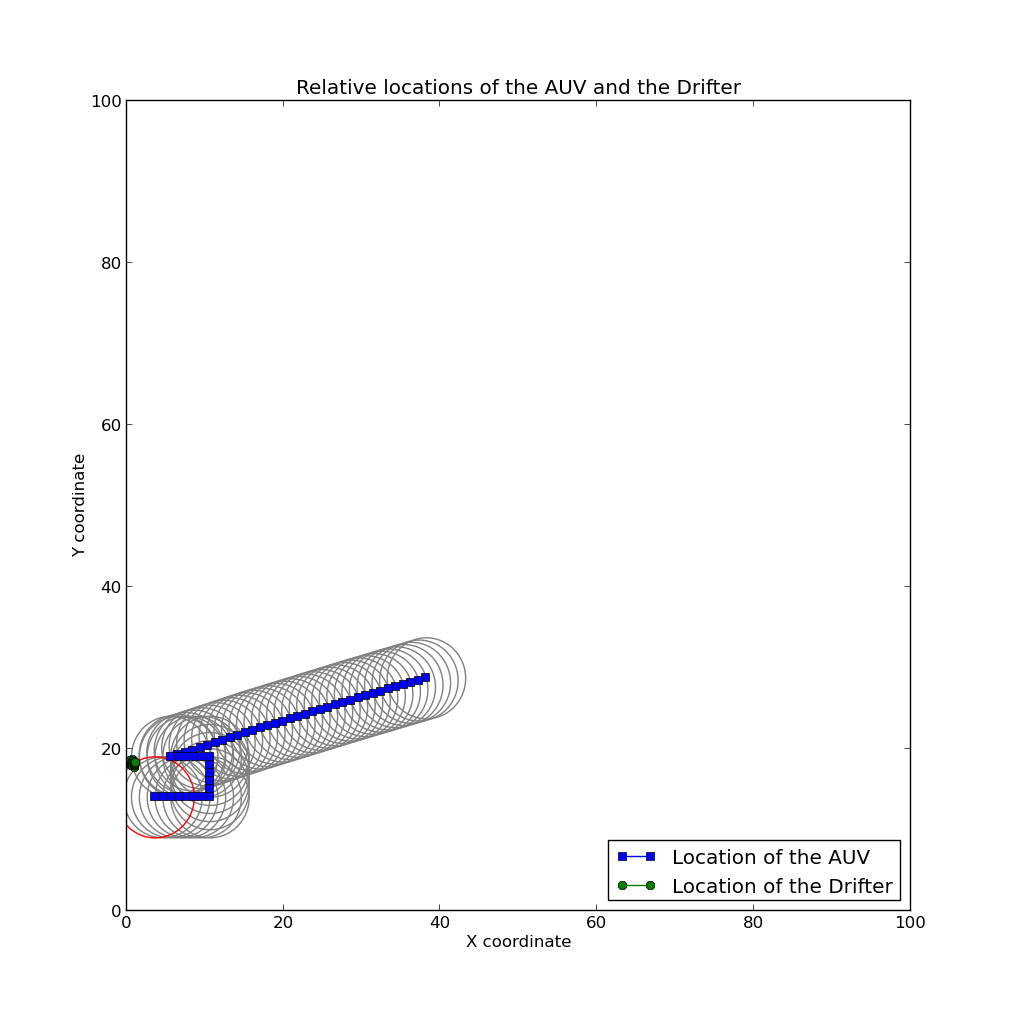
\includegraphics[scale=0.30]{bad_spiral.png}
		\vspace{-20pt}
	\end{center}
\caption{An example of a "bad" spiral which covers area that has already been searched \label{badSpiral}}
\end{figure}

\noindent Not only is our solution not always the most efficient, as mentioned above, but it also occasionally fails to find the drifter altogether. Sometimes the drifter has managed to evade the search pattern by moving into an area that has already been searched, as seen in figure Figures ~\ref{stillMisisng2}, as well as when the drifter is located near the boarders of the search space, as seen in Figure ~\ref{stillMisisng3}. The reason behind this remains to be investigated. These misses occur more often w a smaller communication radius.

\begin{figure}[H]
	\begin{center}
		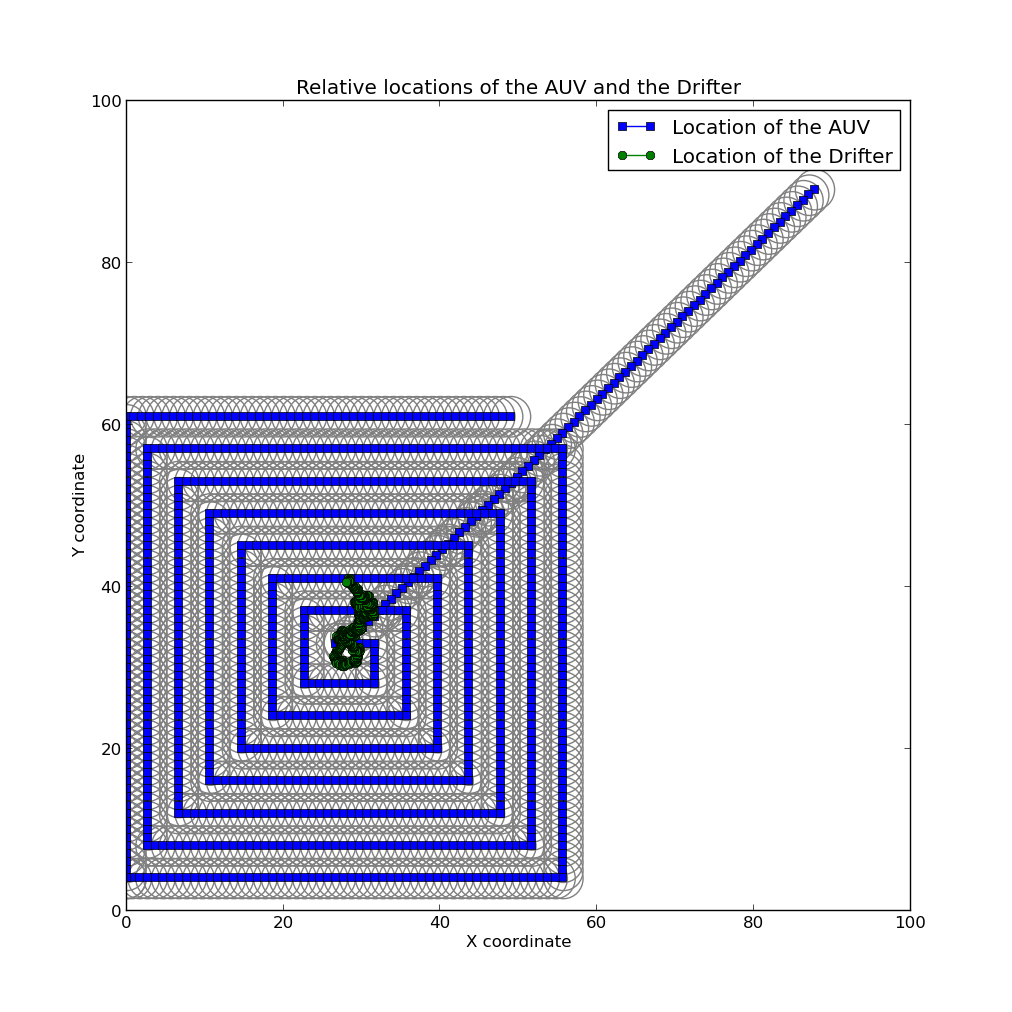
\includegraphics[scale=0.30]{still_missing_2.png}
		\vspace{-20pt}
	\end{center}
\caption{The AUV fails to find the drifter \label{stillMisisng2}}
\end{figure}

\begin{figure}[H]
	\begin{center}
		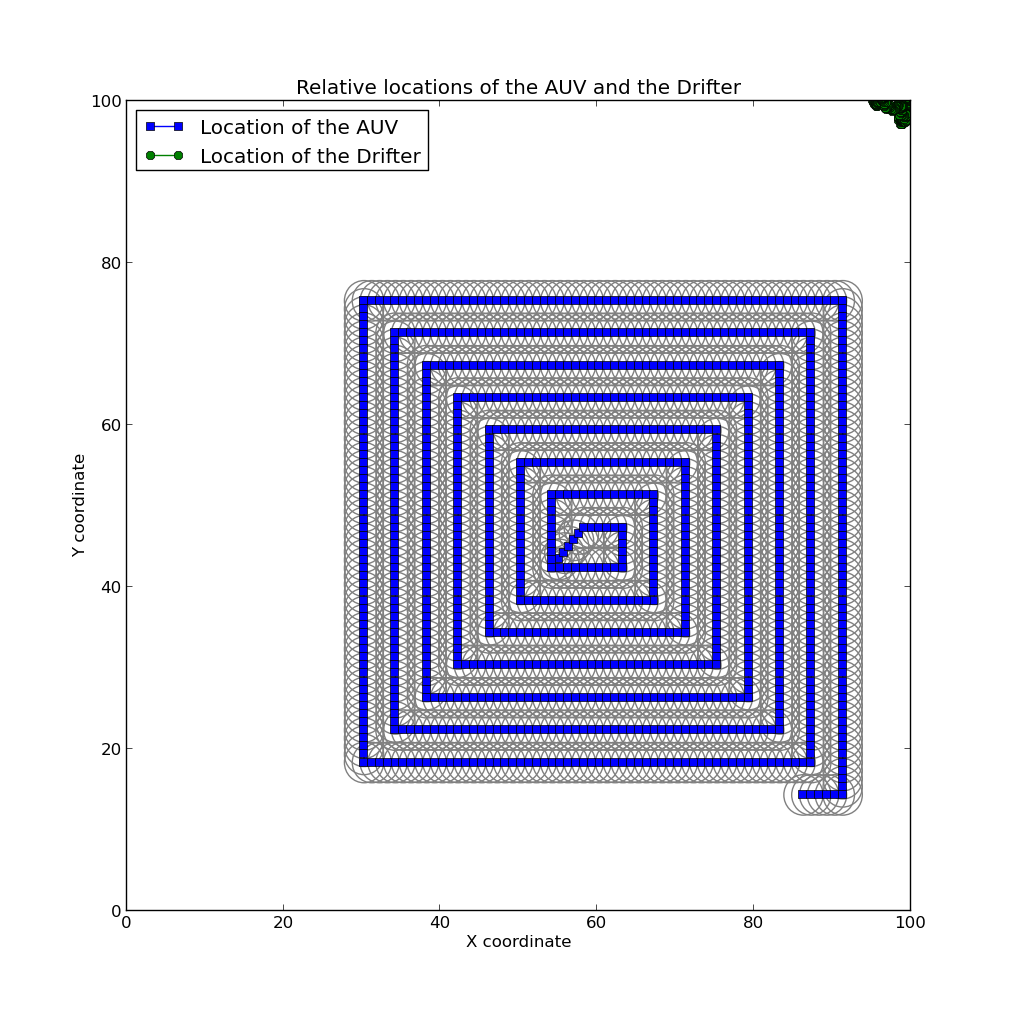
\includegraphics[scale=0.30]{still_missing_3.png}
		\vspace{-20pt}
	\end{center}
\caption{Problem arise when the the drifter is located near the edge of the world (in this case, the upper right hand corner). \label{stillMisisng3}}
\end{figure}

\noindent Though we did not vary the speed of the drifter, it stands to reason that if the speed of the drifter was to increase, we would encounter more cases in which the AUV was unable to find the drifter.

\noindent There might also be a slight disconnect between the absolute distances and the probabilistic grid. The array of floats used to represent the belief state of the AUV is composed of 1 $m$ by 1 $m$ squares. Most of the other calculations used throughout the model use the Euclidean distance. A finer grid may produce better results. \\

\noindent This method, as mentioned previously, is quite basic and leaves room for extension. It is the bare-bones skeleton upon which, ideally, more complex variables can be modelled. While we did implement a square spiral search pattern, it would be interesting to consider the round spiral search patterns mentioned in ~\cite{meghjani14} paired with the appropriate increases in speed. These more mathematically complex geometries might perform better than a square trajectory. It is worth noting that in their exploration of a real-life AUV, Meghjani et al ~\cite{meghjani14} used a square spiral, as opposed to the rounded spiral which they used in their computer simulations. It would also be interesting to assess the performance of inward spirals, which we have not investigated thus far but are also mentioned as a possibility by Meghjani et al ~\cite{meghjani14}, albeit with the caveat that inward spiralling requires that the drifter be within a certain radius and thus is less attractive than outward spiralling.\\

\noindent It might also be interesting to try implementing an AUV with a mass. Currently, our models are independent of mass. The AUV can move in any direction instantaneously - it does not have momentum. In the basic model, the robot never needs to turn because it heads directly to the highest probability location. However, turns are a large part of the spiral search patterns discussed above. A robot with momentum would not be able to make the sharp turns indicated by the Square Spiral model. It would also be prudent to consider an AUV with the ability to accelerate. In this case, the model with the lowest search time would generally be the one that minimized the number of turns. All told, adding mass and acceleration would result in more realistic AUV movement, which would translate into more realistic finding times.\\

\noindent Wind and current also play a role in the movement of the drifter and the AUV, but are not considered in this model. An AUV moving against the current would be forced to move more slowly, and an AUV moving with the current would move more quickly. The analysis carried out by Meghjani et al ~\cite{meghjani14} suggests that as the robot approaches the outer reaches of the spiral, it must increase it's speed accordingly. It would be interesting to see how current would factor into this. Wind and current also affect the drift of the drifter - the drifter would clearly be more likely to drift downwind. Not only is the drift of the drifter impacted, but so is the kernel which the AUV uses to blur its belief state. If the drifter is more likely to drift downwind, it should take this into consideration and adjust the kernel accordingly by weighting the cells that represent "down-wind" more highly.\\ 

\noindent A final interesting addition would be using several drifters. It is entirely reasonable to think that there may be several objects at sea wich the AUV would like to rendezvous with. Not only must it locate each drifter, but it must also plan the most efficient path between the different beacons, taking into account the fact that each drifter moves independently. This combines the current task of locating a free-floating drifter at sea with the well-studied field of path planning. \\
  
\noindent There remains the question of computation time which, while not strictly an evaluation of the method or potential addition still presents a real-world concern. Our model assumes that the robot can perform calculations instantaneously and then move in the correct movement for one second. For small initial distances between the AUV and the drifter this is not a problem. However, with very large search spaces, multiple beacons, spiral search patterns or otherwise increased complexity, the amount of time that the AUV spends computing the location of the drifter becomes non-trivial and must be factored into the calculation of the overall time to find the drifter. Even if this is not a problem in terms of computation time, computational efficiency should at least be considered with regards to battery drain.


%------------------------------------------------

\section*{Conclusion}

The initial models in this paper are based on an AUV that moves at 1 $m/s$ and has a communication radius of 5$m$. This means that if the drifter comes within $5m$ of the boat, it is considered "found". In the most basic model, the average time to find a drifter located approximately 70.0 $m$ away is 64.904 seconds. The time required to find a drifter increases linearly with the size of the initial distance as long as it can find the drifter without needing to use a spiral. However, the time to find the drifter after a spiral search is begun is highly variable and, due to the set pattern of spiral generation (right, down, left, up), is highly dependent on the relative position of the AUV to the drifter. Despite the many improvements that can be made to this model, it seems safe to say that we are now better equipped to find a Wandering Waldo than when we began this investigation!

\newpage
%----------------------------------------------------------------------------------------
%	BIBLIOGRAPHY
%----------------------------------------------------------------------------------------
\bibliographystyle{unsrt} %Used BibTeX style is unsrt
\bibliography{project_bibliography}



%----------------------------------------------------------------------------------------

\end{document}